\chapter{The Algebra of Spacetime}
\label{cha:sta}


Special relativity is geometry with a Lorentzian signature.
The \textdef{spacetime algebra} (STA) is the name given to the geometric algebra of a Minkowski vector space, $\GA(1,3) ≡ \GA(\RR^4, η)$, where $η = ±\op{diag}\sig{-+++}$.
Other introductory material on the STA can be found in \cite{hestenes2003sta,gull1993sta,dressel2015sta}.


We denote the standard vector basis by $\qty{\vb γ_μ}$, where Greek indices run over $\qty{0,1,2,3}$.
This is a deliberate allusion to the Dirac $γ$-matrices, whose algebra is isomorphic to the STA --- however, the $\vg_μ ∈ \RR^{1+3}$ of STA are real, genuine spacetime vectors.
A basis for the entire $2^4$-dimensional STA is then
\begin{fullwidth}
	\newcommand{\below}[2]{\underset{#1}{\vphantom{\int}#2}}
	\begin{align}
		\overset{\text{1 scalar}}{
			\set[\big]{ \below{+}{\vb 1} }
		}
	∪	\overset{\text{4 vectors}}{
			\set[\big]{ \below{+}{\vg_0}, \; \below{-}{\vg_i}}
		}
	∪	\overset{\text{6 bivectors}}{
			\set[\big]{ \below{+}{\vg_0\vg_i}, \; \below{-}{\vg_j\vg_k}}
		}
	∪	\overset{\substack{\text{4 trivectors}}}{
			\set[\big]{ \below{-}{\vg_0\vg_j\vg_k}, \; \below{+}{\vg_1\vg_2\vg_3}}
		}
	∪	\overset{\substack{\text{1 pseudoscalar}}}{
			\set[\big]{ \vol ≔ \below{-}{\vg_0\vg_1\vg_2\vg_3}}
		}
	\end{align}
\end{fullwidth}
where lowercase Latin indices range over spacelike components, $\set{1,2,3}$.
Blades shown on the left-hand side of $\set{\quad,\quad}$ are called \textdef{timelike}, and those in on right-hand side \textdef{spacelike}.
The sign below each basis blade shows its signature (the sign of its scalar square).
Multivectors of any kind which square to zero are called \textdef{null}.


\subsubsection{The pseudoscalar and duality}

The right-handed unit pseudoscalar $\vol$ represents an oriented unit $4$-volume.
It anticommutes with odd elements of the STA (vectors and trivectors) and commutes with even elements (bivectors and \paren{pseudo}scalars).

Since $\vol^2 = -1$, the scalar--pseudoscalar plane $\GA[0,4](1,3) = \op{span}_\RR\set{1, \vol}$ is isomorphic to the complex plane $\CC$.
Thus, for the sake of computation, operations on $\set{0, 4}$-multivectors may be regarded as operations on complex numbers.
In particular, we define the principal root $\sqrt{a}$ of a $\set{0,4}$-multivector $a ∈ \GA[0,4](1,3)$ in the same way as it is defined in $\CC$ with a branch cut at $θ = π$.
It is worth emphasising that there are many square roots of $-1$ in the spacetime algebra, each with distinct geometrical meanings.\sidenote{
	E.g., the spacelike bivector $(\vg_i\vg_j)^2 = -1$ represents a directed spacelike plane.
	% ; the timelike vector $\vg_0^2 = -1$ a particle's velocity.
	% METRIC-SENSITIVE
}
We single to single out $\sqrt{-1} = \vol$ as `the' principal root as this proves to be useful notationally.\sidenote{
	In electromagnetism, the imaginary unit $i$ often represents the volume element $\vol$.
	E.g., in the Riemann--Silberstein vector \cite{silberstein}, both $i$ and $\vol$ play roles similar to the Hodge dual \cite{dressel2015sta}.
}

As in \cref{sec:ga-hodge-dual}, Hodge duality is accomplished by (right) multiplication by the volume element.
In particulat, this establishes a duality between vectors and trivectors, and between spacelike and timelike bivectors.

\section{The space/time Split}
\label{sec:spacetime-split}

While we actually live in $\RR^{1,3}$ spacetime, to any particular observer it appears that space is $\RR^3$ with a separate scalar time parameter.
This is reflected in the fact that $\GA[+](1,3)$ and $\GA(3)$ are isomorphic, from \cref{lem:even-subalg-isos}.
In fact, there is a separate isomorphism associated to each timelike direction, corresponding to each inertial observer's personal spacetime split.
Such a \textdef{space\slash time split} identifies \emph{even} multivectors in the spacetime algebra $\GA[+](1,3)$ with $\GA(3)$ multivectors, providing an efficient, purely algebraic method for switching between inertial frames \cite{hestenes2003sta}.


Let $K$ be an inertial observer and for simplicity choose the standard basis $\qty{\vg_μ}$ so that $\vg_0$ is the instantaneous velocity of the $K$ frame.
The three \textdef{relative vectors} $\vs_i ≔ \vg_i\vg_0$ form a vector basis for $\GA(3)$, since the $\vg_i\vg_0$ indeed satisfy $\vs_i^2 = -\vg_i^2\vg_0^2 = 1$ and $\vs_i\vs_j = -\vs_j\vs_i$ for $i ≠ j$.
Because of the dependence on the frame's velocity vector $\vg_0$, the relative vectors $\vs_i$ are particular to the $K$ frame.
With respect to the $K$ frame, we may view $\GA(3) ⊂ \GA(1,3)$ as embedded in the STA, allowing us to consider multivectors as belonging to both spaces.
Note that the same volume element $\vol = \vs_1\vs_2\vs_3 = \vg_0\vg_1\vg_2\vg_3$ is shared by the algebras.

For example a spacetime bivector $F = F^{μν}\vg_μ\vg_ν$ may be separated into timelike $F^{i0}$ and spacelike $F^{ij}$ components with respect to the $K$ frame and viewed as a $\qty{1,2}$-multivector in $\GA(3)$,
\begin{align}
	\label{eqn:sta-bivector-split}
	F = F^{i0}\vg_i\vg_0 + F^{ij}\vg_i\vg_j
	= E^i\vs_i + B^i\vol\vs_i = \vec E + \vol \vec B
,\end{align}
where we use
\begin{math}
	\vg_i\vg_j
	= (\vg_i\vg_0)(\vg_j\vg_0)
	= -\vs_i\vs_j
	= -ε_{ijk}\vol\vs_k
.\end{math}
Note that the relativistic representation $F$ is \emph{equal} to the frame-dependent representation --- they are the same spacetime object.
\Cref{eqn:sta-bivector-split} performs the frame-dependent decomposition of a spacetime bivector (or ``2-form'') into two $\RR^3$ vectors familiar from electromagnetic theory.


Of particular interest are space\slash time splits on bivector generators associated to rotors.
A proper orthochronous Lorentz transformation $\lin Λ ∈ \SO^+(1,3)$ acts as a `sandwich' product $\lin Λ(A) = e^σ A e^{-σ}$, where the rotor $e^σ \in \op{Spin}^+(1,3)$ is generated by a spacetime bivector $σ ∈ \GA[2](1,3)$.
This bivector $σ$ can be represented in the $K$ frame as
\begin{align}
	σ = \frac12(ξ^i \vg_i + θ^i \vol \vg_i)\vg_0
	= \frac12(\vb ξ + \vol \vb θ)
	\label{eqn:bivector-generator}
\end{align}
where $\vb ξ = ξ^i\vs_i ∈ \GA[1](3)$ is a rapidity vector and $\vol \vb θ ∈ \GA[2](3)$ is a rotation bivector.


\subsection{On the choice of metric signature}

Both metric signatures $η = \op{diag}\sig{-+++}$ and $η = \op{diag}\sig{+---}$ are appropriate for relativistic physics, and both are used in the literature.
While the overall physics is agnostic to this choice, expressions written in the STA are generally not independent of the overall sign.
It is a useful reference to note what changes and what is constant under both choices.

One of the most important properties of the space\slash time split is the union of the $\GA(3)$ and $\GA[+](1, 3)$ volume elements, $\vol = \vs_1\vs_2\vs_3 = \vg_0\vg_1\vg_2\vg_3$.
If this equality is to hold, then switching the metric signature is concomitant with a switch in sign of the relative vectors, $\vs_i ↦ -\vs_i$. 
Another noticable difference is in the space\slash time split of a position vector $𝑿 ∈ \GA[1](1, 3)$ into components $𝑿^0 = ct$ and $(𝑿^i) = \vec x$, achieved by multiplication with the frame velocity $\vg_0$.
For example, the equations
\begin{align}
	𝑿 \vg_0 &= ct + \vec x
,&	\vg_0 𝑿 &= ct - \vec x
\end{align}
hold in the $\sig{+---}$ signature, but both change by an overall sign in the $\sig{-+++}$ signature.\sidenote{
	In all cases, reversion $𝑿 \vg_0 ↦ \rev{(𝑿 \vg_0)} = \vg_0 𝑿$ simply negates the spacetime bivector part, $\vec x → -\vec x$.
}
Both these points are summarised in \cref{tbl:sig-choice}.

\begin{table}[h]
	\centering
	\renewcommand{\arraystretch}{1.15}
	\begin{tabular}{CCCCCC}
		\emph{signature} & \emph{preferred $\vs_i$}
			& \vg_0 𝑿 & 𝑿 \vg_0
	\\ \hline
		\sig{+---} & \vs_i ≔ \vg_i\vg_0
		& \phantom{+}ct - \vec x & \phantom{+}ct + \vec x

	\\	\sig{-+++} & \vs_i ≔ \vg_0\vg_i
		& -ct + \vec x & -ct - \vec x
	\end{tabular}
	\caption{
		Comparison of space\slash time split in each metric signature.
		The spacetime vector $X$ has contravariant components $X^0 = ct$ and $(X^i) = \vec x$ in the $\vg_0$-frame.
		Relative vectors are defined so that the spacetime volume element and volume element under a space\slash time split are equal.
	}
	\label{tbl:sig-choice}
\end{table}

A choice of metric sign may be avoided by using sign-agnostic expressions.
An invariant definition of relative vectors and their duals in the $\vg_0$-frame is
\begin{align}
	\vs_i &≔ \vg_i\vg^0
,&	\vs^i &= \vg_0\vg^i
.\end{align}
These satisfy $\vol = \vs_1\vs_2\vs_3 = \vg_0\vg_1\vg_2\vg_3$ and
$\vol^{-1} = \vs^1\vs^2\vs^3 = \vg^0\vg^1\vg^2\vg^3$ in either signature.
In particular, the following expressions hold in either signature, and are useful when performing space\slash time splits.
\begin{align}
	\vg^0 𝑿 &= ct - \vec x
&	𝑿 \vg^0 &= ct + \vec x
\\	\vg_0 \, \vd &= \frac1c \pdv{t} + \vec ∇
&	\vd \, \vg_0 &= \frac1c \pdv{t} - \vec ∇
\end{align}
Here, the spacetime vector derivative $\vd = \vg^μ ∂_μ$ decomposes into a scalar time derivative $∂_0 = c^{-1}∂_t$ and the spatial derivative $\vec ∇ = \vs^i ∂_i$.


\section{The Invariant Bivector Decomposition}
\label{sec:invariant-bivector-decomposition}

There is a clear analogy between the space\slash time split of a bivector \eqref{eqn:sta-bivector-split}, into spacelike and timelike components, and the Cartesian form of a complex number, $x + iy$, into real and imaginary parts.
This similarity can be made more precise: just as we may express complex numbers in polar form $re^{iϕ} = x + iy$, we may use the invariant bivector decomposition to write $ρe^{\vol σ} = E + \vol B$, since $\vol^2 = i^2 = -1$.
This is distinct from the space\slash time split in that it is frame \emph{independent}, and the bivector $E$ is not necessarily timelike, and so need not correspond to any relative vector $\vec E ∈ \GA[1](3)$.


Non-null spacetime bivectors $σ \in \GA[2](1,3)$ may be \emph{normalised}, in the sense that there always exists some $N_σ \in \GA[0,4](1,3)$ such that
\begin{align}
	σ = N_σ\hat{σ} = \hat{σ}N_σ
	\qqtext{where}
	\hat{σ}^2 = 1
.\end{align}
In the null case $σ^2 = 0$, we let $\hat{σ}^2 = 0$ instead.
This is possible because the square of a bivector is a $\set{0, 4}$-multivector (\cref{lem:grades-of-square}), which always has a principle square root (since $\GA[0,4](1,3) ≅ \CC$).
Explicitly, let $σ^2 = α + \vol β = ρ^2e^{2\vol ϕ}$ for scalars $α, β, ρ, ϕ$, so that
\begin{align}
	N_σ
	\coloneqq \sqrt{σ^2}
	= ρe^{\vol ϕ}
	\label{eqn:spacetime-bivector-normaliser}
,\end{align}
assuming without loss of generality that $ρ > 0$ and $ϕ \in (-π/2, π/2]$.
Thus, the \textdef{invariant bivector decomposition}
\begin{align}
	\label{eqn:invariant-bivector-decomposition}
	σ = ρe^{\vol ϕ}\hat{σ}
	&= \underbrace{(ρ\cos ϕ)\hat{σ}}_{σ_+} + \underbrace{(ρ\sin ϕ)\vol\hat{σ}}_{σ_-}
\end{align}
separates $σ$ into commuting parts, $[σ_+, σ_-] = 0$, each of which satisfy $±σ_±^2 > 0$.
This makes it a useful device for algebraic manipulations.
Furthermore, the decomposition is unique, and does not depend on any particular space\slash time split.



The decomposition can be used to show the non-injectivity of the exponential map in the STA.
Take some bivector written in decomposed form,
\begin{math}
	σ = λ_+\hat σ + λ_-\vol\hat σ
.\end{math}
For $n ∈ \ZZ$, each bivector in the family
\begin{align}
	σ_{n} = λ_+\hat σ + (λ_- + nπ)\vol\hat σ
	\label{eqn:equivalent-generators}
\end{align}
exponentiates to the same rotor, up to an overall sign: 
\begin{align}
	e^{σ_{n}} = e^{σ_{0}}e^{nπ\vol\hat σ} = (-1)^ne^{σ_{0}}
	\label{eqn:equivalent-rotors}
\end{align}
Note that $e^{\hat σ + \vol\hat σ} = e^{\hat σ}e^{\vol\hat σ}$ since $[\hat σ, \vol\hat σ] = 0$.
All the rotors in \cref{eqn:equivalent-rotors} correspond to the same $\SO^+(1,3)$ Lorentz transformation.
\Cref{eqn:equivalent-rotors} shows that every Lorentz rotor $±e^{σ_0}$ is equal to a pure bivector exponential $e^{σ_n}$ with a shifted rotational part $λ_- \mapsto λ_- + n\pi$.


\section{Lorentz Conjugacy Classes}

As shown above, every proper Lorentz transformation $\lin Λ ∈ \SO^+(1, 3)$ is generated by a bivector exponential $\lin Λ(𝒖) = e^σ 𝒖 e^{-σ}$.
This rotor formulation of the Lorentz group makes some of its more subtle properties clear, including its decomposition into conjugacy classes.
\begin{definition}
	The \textdef{conjugacy class} of a group element $g ∈ G$ is the set
	\begin{align}
		[g] ≔ \set{hgh^{-1} | h ∈ G} = \set{g' ∈ G | g' \sim g}
	\end{align}
	of elements conjugate\sidenote{
		Group elements $g \sim g'$ are conjugate iff there extists $h ∈ G$ such that $g = hg'h^{-1}$.
	} to $g$.
\end{definition}
Since conjugacy is an equivalence relation, the conjugacy classes partition the group $G$.

In the case of the proper Lorentz group, the set of conjugacy classes further partitions into five categories, or `kinds', according to basis-invariant properties of the constituent Lorentz transformations.
Using the STA, the `kind' of a Lorentz transformation (or of its associated rotors) is given by basic properties of its generating bivector.\sidenote{
	One rotor has many generating bivectors, but any one will do.
}

\begin{definition}
	\label{def:lorentz-kinds}
	Let $σ ∈ \GA[2](1, 3)$ be a bivector.
	If $σ^2$ is a scalar, then $σ$ is called
	\begin{itemize}
		\item \textdef{trivial} if $σ = 0$; and if $σ ≠ 0$,
		\item \textdef{elliptic} if $σ^2 < 0$;
		\item \textdef{parabolic} if $σ^2 = 0$;
		\item \textdef{hyperbolic} if $σ^2 > 0$; and
		\item \textdef{loxodromic} if $σ^2 = α + \vol β$ is not a scalar but a $\set{0, 4}$-multivector.
	\end{itemize}
	% If $σ^2 = α + \vol β$ is not a scalar but a $\set{0, 4}$-multivector, then call $σ$ \textdef{loxodromic}.
\end{definition}

\begin{lemma}
	The square of a bivector is constant within each conjugacy class.
\end{lemma}
\begin{proof}
	Let $\lin Λ : 𝒖 ↦ e^σ 𝒖 e^{-σ}$ be a proper Lorentz transformation, and consider its conjugation with some other transformation $\lin Γ$,
	\begin{align}
		\lin{Γ Λ Γ}^{-1} : 𝒖 ↦ e^ρ e^σ e^{-ρ} 𝒖 e^{-ρ} e^{-σ} e^ρ
	.\end{align}
	Note that
	\begin{math}
		e^ρ e^σ e^{-ρ} =  e^{e^ρ σ e^{-ρ}}
	\end{math}
	by the automorphism property of rotor application.
	Therefore, conjugacy of $\lin Λ \sim \lin{Γ Λ Γ}^{-1}$ translates to bivectors as
	\begin{align}
		σ \sim σ' ≔ e^ρ σ e^{-ρ}
	\end{align}
	for some $ρ$.
	Hence, the conjugate bivectors have common square,
	\begin{align}
		σ'^2 = (e^ρ σ e^{-ρ})^2 = e^ρ σ^2 e^{-ρ} = σ^2
	\end{align}
	since $e^{±ρ}$ commutes with the $\set{0, 4}$-multivector $σ^2$.
\end{proof}

\begin{corollary}
	Conjugacy classes of $\SO^+(1, 3)$ fall into the five categories in \cref{def:lorentz-kinds} by considering the generating bivector of any representative Lorenz rotor.
\end{corollary}


\begin{marginfigure}
	\centering
	\begin{subfigure}{\columnwidth}
		\centering
		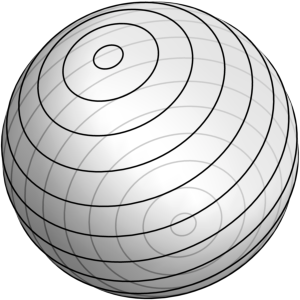
\includegraphics[width=.7\columnwidth]{figures/celestial-ball-1.pdf}
		\caption{Elliptical}
	\end{subfigure}
	\vskip3ex
	\begin{subfigure}{\columnwidth}
		\centering
		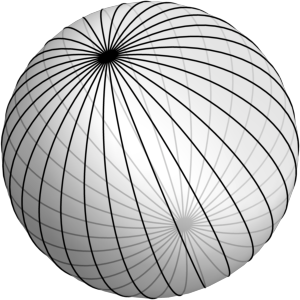
\includegraphics[width=.7\columnwidth]{figures/celestial-ball-2.pdf}
		\caption{Hyperbolic}
	\end{subfigure}
	\vskip3ex
	\begin{subfigure}{\columnwidth}
		\centering
		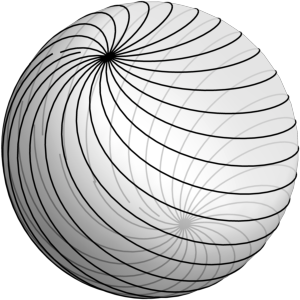
\includegraphics[width=.7\columnwidth]{figures/celestial-ball-3.pdf}
		\caption{Loxodromic}
	\end{subfigure}
	\caption{
		Lorentz transformations on the celestial sphere, taking curves to themselves.
	}
	\label{fig:celestial-balls}
\end{marginfigure}


Elliptical Lorentz transformations are \emph{rotations}, whose rotors are generated by spacelike $2$-blades; hyperbolic transformations are \emph{boosts}, with timelike $2$-blades generators.
Parabolic transformations are sometimes called \emph{null rotations}, and fall in between the previous two, with null $2$-blades as generators.

The final class of loxodromic transformations are a combination of a rotation and a boost where the axis of rotation is parallel with the boost direction (in a particular frame).
A loxodromic generator is \emph{not} a $2$-blade, but a bivector comprising mutually $2$-orthogonal\sidenote{
	in the sense of \cref{def:Δ-orthogonal}, \cref{sec:higher-orthogonal}
} $2$-blades, one timelike and one spacelike.

These can be helpfully visualised by making use of the isomorphism $\SO^+(1,3) \cong \op{Aut}(\CC \cup \set{∞})$ of the Lorentz group with the Möbius group of conformal transformations on the sphere.
An observer undergoing a change of frame will see the celestial sphere transform conformally, as in \cref{fig:celestial-balls}.